\section{函数}

\begin{frame}
  \begin{biancheng}
    设计函数\lstinline|min(x, y)|,返回两个\lstinline|double|数值中的较小值,并测试之。
  \end{biancheng}
\end{frame}

\begin{frame}
  \begin{biancheng}
    编写一个函数,打印一个字符矩阵,需要三个参数,即一个字符和两个整数,其中
    \begin{itemize}
    \item 字符参数是需要输出的字符
    \item 第一个整数为矩阵的行数
    \item 第二个整数为矩阵的列数
    \end{itemize}
  \end{biancheng}
\end{frame}

\begin{frame}
  \begin{biancheng}
    编写一个函数,判断某一年是否为闰年。闰年的判断条件为:
    \begin{enumerate}
    \item 能够被4整除却不能被100整除的数。
    \item 能够被400整除的数。
    \end{enumerate}
  \end{biancheng}
\end{frame}

\begin{frame}
  \begin{biancheng}
    已知三角形的三个顶点为$(x_1,y_1), (x_2, y_2), (x_3, y_3)$,编写一个函数求三角形的面积,其中面积公式为
    $$
    S = \left|
      \begin{array}{ccc}
        1&1&1\\
        x_1&x_2&x_3\\
        y_1&y_2&y_3
      \end{array}
    \right|
    $$
  \end{biancheng}
\end{frame}

\begin{frame}
  \begin{biancheng}
    编写一个递归函数\lstinline| power() |,用于计算一个double数的某正整数次幂。
  \end{biancheng} \pause 

  $$
  a^n = \left\{
    \begin{array}{ll}
      1, & n = 0, \\[.1in]
      \left(a^{\left\lfloor \frac n2 \right\rfloor}\right)^2 \times a, & n \mbox{ odd }, \\[.1in]
      \left(a^{\left\lfloor \frac n2 \right\rfloor}\right)^2 , & n \mbox{ even }
    \end{array}
  \right.
  $$
\end{frame}

\begin{frame}
  \begin{biancheng}
    回顾十进制转二进制的函数\lstinline| to_binary() |,然后思考一下如何对其进行推广,将某个十进制数转换为任意进制,即构造一个新的函数\lstinline| dec2base() |。如\lstinline|dec2base(129, 16)|的输出为\lstinline|7F|,即\lstinline|129|的十六进制数。
  \end{biancheng}
\end{frame}

\begin{frame}
  \begin{biancheng}
    传说婆罗门庙里有一个塔台,台上有3根标号为A、B、C的用钻石做成的柱子,在A柱上放着64个金盘,每一个都比下面的略小一点。把A柱上的金盘全部移到C柱上的那一天就是世界末日。移动的条件是:
    \begin{itemize}
    \item 一次只能移动一个金盘;
    \item 移动过程中大金盘不能放在小金盘上面。
    \end{itemize}
    庙里的僧人一直在移个不停,移动的最少总次数是$2^{64}-1$次,如果每秒移动一次的话,需要500亿年。
  \end{biancheng}
\end{frame}

\begin{frame}
  \begin{itemize}
  \item 若$n=1$,则将这一个盘子直接从A柱移动到C柱上,最少移动$2^1-1=1$次。
  \item 若$n>1$,则执行以下3步,最少移动$2^n-1$次:
    \begin{enumerate}
    \item 借助C柱,将A柱上的$n-1$个盘子移到B柱;\\[.1in]
    \item 将A柱上最后一个盘子直接移到柱;\\[.1in]
    \item 借助A柱,将B柱上的$n-1$个盘子移到C柱。
    \end{enumerate}
  \end{itemize}
\end{frame}

\begin{frame}
  \begin{figure}[htbp]
    \centering
    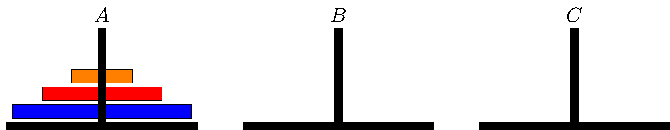
\includegraphics[width=4in]{ch09/images/ht0.pdf}
  \end{figure}
\end{frame}

\begin{frame}
  \begin{figure}[htbp]
    \centering
    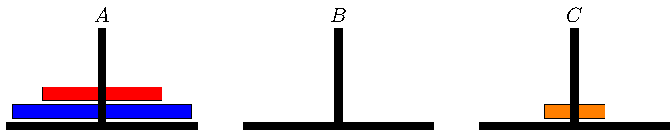
\includegraphics[width=4in]{ch09/images/ht1.pdf}
  \end{figure}
\end{frame}

\begin{frame}
  \begin{figure}[htbp]
    \centering
    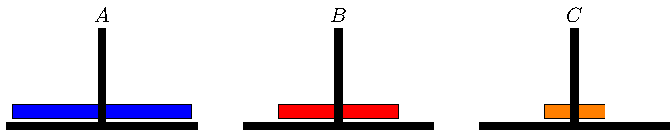
\includegraphics[width=4in]{ch09/images/ht2.pdf}
  \end{figure}
\end{frame}

\begin{frame}
  \begin{figure}[htbp]
    \centering
    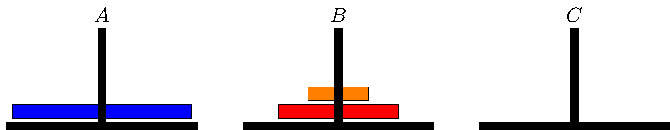
\includegraphics[width=4in]{ch09/images/ht3.pdf}
  \end{figure}
\end{frame}

\begin{frame}
  \begin{figure}[htbp]
    \centering
    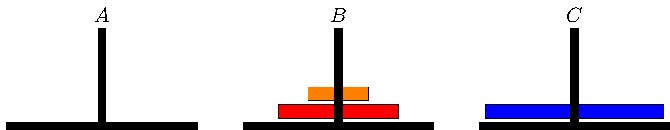
\includegraphics[width=4in]{ch09/images/ht4.pdf}
  \end{figure}
\end{frame}

\begin{frame}
  \begin{figure}[htbp]
    \centering
    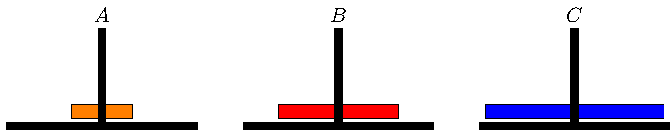
\includegraphics[width=4in]{ch09/images/ht5.pdf}
  \end{figure}
\end{frame}

\begin{frame}
  \begin{figure}[htbp]
    \centering
    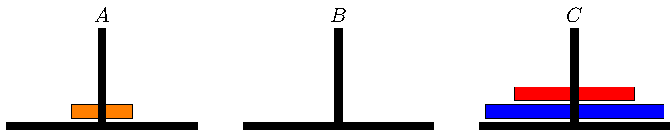
\includegraphics[width=4in]{ch09/images/ht6.pdf}
  \end{figure}
\end{frame}

\begin{frame}
  \begin{figure}[htbp]
    \centering
    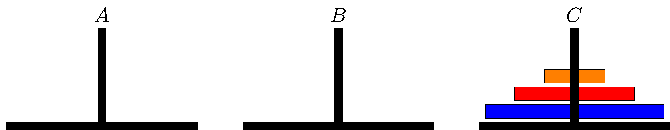
\includegraphics[width=4in]{ch09/images/ht7.pdf}
  \end{figure}
\end{frame}
